\documentclass[12pt]{article}
\usepackage{graphicx,url,placeins,algorithm,algorithmic,amsmath,subfigure}
\usepackage[hidelinks]{hyperref}
\usepackage[titletoc]{appendix}
%\usepackage{pdfpages}
\usepackage{listings}
%\usepackage{layout}
\usepackage[font=small,labelfont=bf]{caption}
\usepackage[utf8]{inputenc}
\graphicspath{{figures/}}
\setlength{\voffset}{0in}
\setlength{\headsep}{5pt}
\addtolength{\textheight}{2cm}
\setlength{\footskip}{5pt}
%
\begin{document}

\title{\vskip -6em TNM084\\Interactive procedural terrain in OpenGL}   % type title between braces

\author{
 Johan Beck-Nor\'{e}n, johbe559@student.liu.se
 }
        \date{\today}    % type date between braces
        \maketitle
        
\section{Background}
For this project I created procedurally generated terrain. Terrain can be cumbersom to create by hand with explicitly defined geometry. It is a complex structure and can take a lot of time and effort to produce a convincing terrain geometry. Because of this procedural methods is a good and widely used method when creating large terrain geometry in computer graphics. For this project I have used an implementation of 2D simplex noise implemented in GLSL by Stefan Gustavsson [https://github.com/ashima/webgl-noise]. Using and combining simplex noise of different frequencies applies very well to terrain since terrain often have huge low-frequency variations such as peaks and valleys, as well as finer details of higher frequencies such as smaller hills and hollows. We achieve this by Fractional Brownian Motion (eq. \ref{eq:fbm}). This fits well since the variations of terrain is somewhat fractal in nature, with small hills on top of bigger hills etc.

\begin{equation}
\sum^{\text{num octaves}-1}_{i=0}noise(\vec{v}*freq_i)*amp_i
\label{eq:fbm}
\end{equation}

In eq. \ref{eq:fbm} $\vec{v}$ is a two-dimensional vector, \textit{noise} is the 2D simplex noise function, $amp_i$ is the desired amplitude of the contribution to the final result by frequency $freq_i$. For this project we typically used an amplitude of $\frac{1}{2} amp_{i-1}$ for $amp_i$, and a $freq_i$ of $2*freq_{i-1}$. Manipulating the frequency by a factor of 2 is often referred to as using different octaves of that frequency.

The terrain structure is created by displacing a flat vertex grid along one axis, similar to how one would use a heightmap for the same purpose. The displacement amount for each vertex is determined by eq. \ref{eq:fbm}. The normals are calculated in the same fashion, with the addition of using finite differences to approximate the surface derivatative at the vertex position. We do this by sampling the noise function at four points near the sample point $\vec{v}$, two points along each of the two axes $u$ and $v$. The partial derivatives are calculated as in eq. \ref{eq:normals}.

\begin{equation}
\begin{split}
\frac{\partial noise}{\partial u} = \frac{noise(u+du, v)-noise(u-du,v)}{2*du} \\
\frac{\partial noise}{\partial v} = \frac{noise(u, v+dv)-noise(u,v-dv)}{2*dv}
\label{eq:normals}
\end{split}
\end{equation}

In the equation the vector $\vec{v}$ is represented by $(u,v)$, and $du$ and $dv$ are small scalar numbers denoting the distances at which to sample for the derivatives relative to $u$ and $v$ respectively.
 
\section{Implementation}
The project was implemented in C++ using the OpenGL graphics API and GLSL shaders, along with the GL extension libraries GLEW and GLFW. During the startup of the program a uniform vertex grid is created on the CPU. We send vertex positions to the vertex shader, as well as the grid dimensions, desired number of octaves for the Fractional Brownian Motion, camera position, and matrices needed for transformation and projection to the shader as uniforms. Sending these as uniforms allows us to modify the values during runtime which is valuable when we want to interact and affect the terrain generated. The interaction parameters include:

\begin{enumerate}
  \item Movements forward, back, left, right.
  \item Number of octaves to use when displacing the vertex positions.
  \item Water level.
  \item Free-flying camera
\end{enumerate}

As mentioned we send the camera position explicitly to the vertex shader. When the program is running we calculate the camera transformations as if we were moving around in the scene as well as for a static camera. The reason for this is the way we move around our terrain. We actually keep the camera static, and instead use the calculated camera position sent to the vertex shader to displace the seed to the noise function. Since the noise function is deterministic this work very well and gives the illusion that we are moving over the terrain, when in reality we are only adjusting the seed to the noise funtion. I also implemented a free-fly camera functionality which allows us to detach from the static camera position and view grid from the ``outside''.

The rendering of the terrain is simple. A single directional light source is used, and the terrain color is determined by the height value of the fragment. The water surface if created by clamping the vertex positions to a set threshold value along the Y-axis. We keep the original normal vector for the clamped vertices since this give a bit more interesting texture to the water surface.

\section{Results}
The initial values for the terrain generation are to use 6 octaves for the Fractional Brownian Motion and a water level of $0.4$ with the terrain height values normalized to the interval [0,1]. With these values we get a resuls as in fig. \ref{fig:terrain_init}.

\begin{figure}[h]
	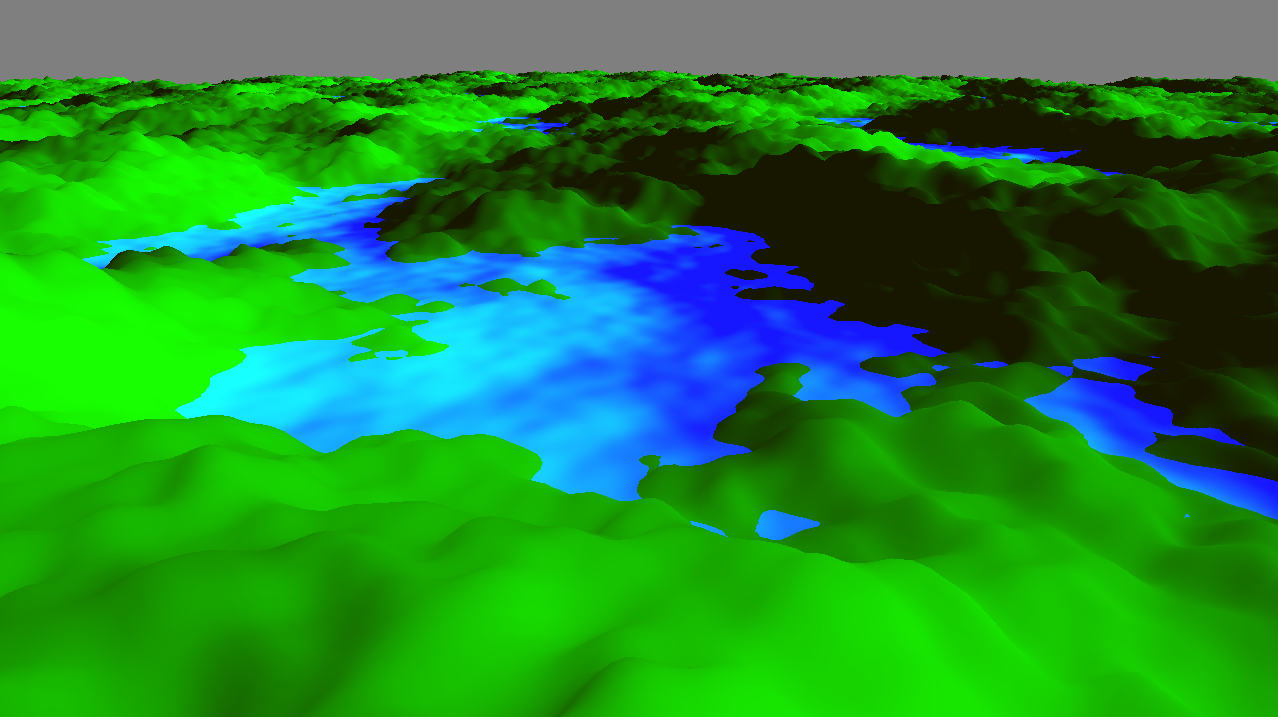
\includegraphics[width=\textwidth]{terrain_init.png}
	\centering
	\caption{Terrain geometry created by displacing a vertex grid with 2D simplex noise using 6 octaves of Fractional Brownian Motion.}
	\label{fig:terrain_init}
\end{figure}

We can adjust some values during runtime. If fig. \ref{fig:octaves} we see the result of increasing the number of octaves used from top to bottom.


\begin{figure}
\centering     %%% not \center
\subfigure[1 octave]{\label{fig:a}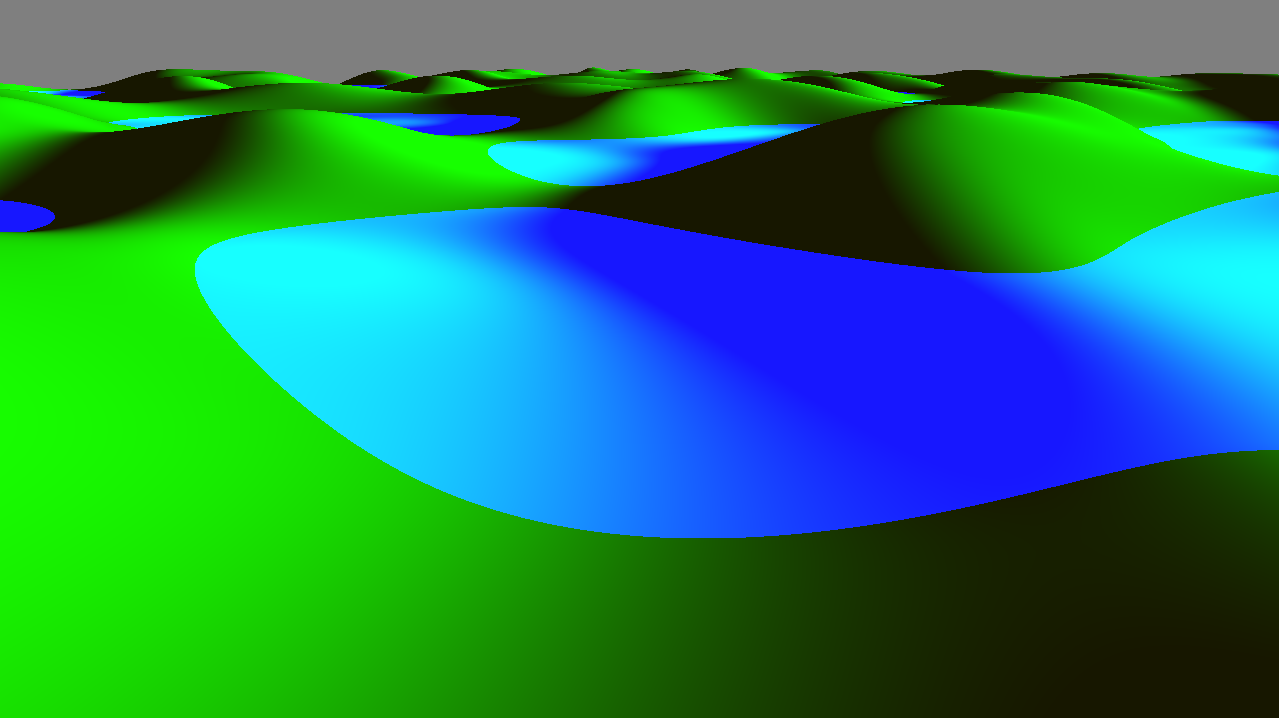
\includegraphics[width=0.7\textwidth]{terrain_1_octave.png}}
\\
\subfigure[4 octaves]{\label{fig:b}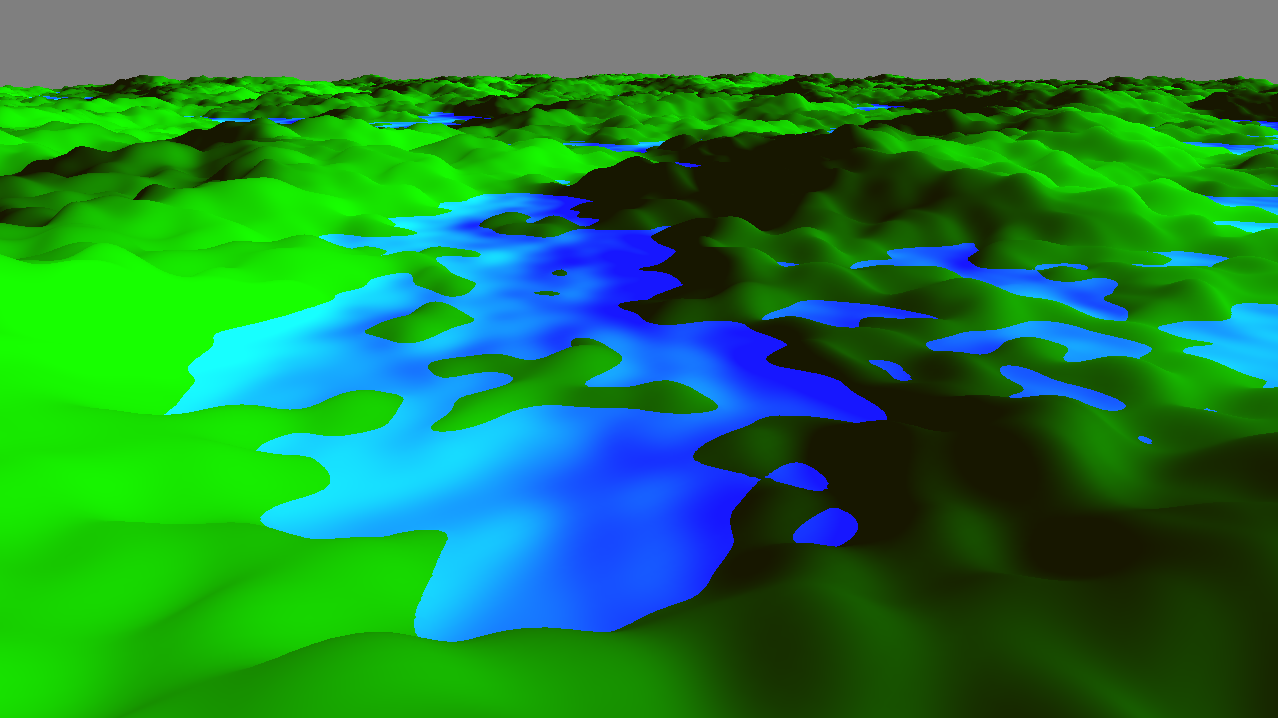
\includegraphics[width=0.7\textwidth]{terrain_4_octave.png}}
\\
\subfigure[8 octaves]{\label{fig:b}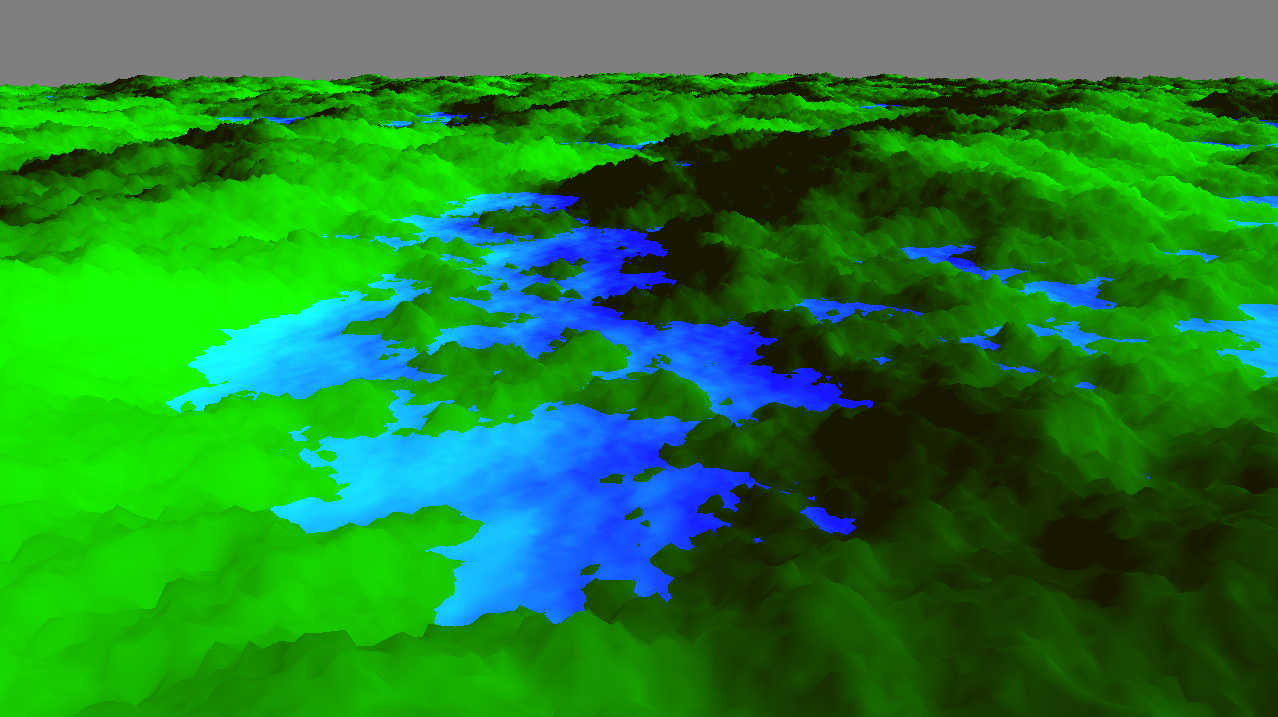
\includegraphics[width=0.7\textwidth]{terrain_8_octave.png}}
\caption{Images showing how using different number of octaves for the Fractional Brownian Motion affect the terrain generated.}
\label{fig:octaves}
\end{figure}

\section{Comments}
Discuss the use of a texture generated on the CPU vs sampling the noise function in the shaders. Also mention the trial with tessellation here maybe.

%\begin{enumerate}
%  \item Stefan Gustavssons implementation of 2D simplex noise in GLSL
%  \item Statiskt vertex grid + statisk cam, camerapos som seed till noisefunc, displace i Y-led mha noise
%  \item Ytnormaler för den displacade ytan beräknas mha finita differenser (partiella derivator) i vertex shadern.
%  \item Implementerat i OpenGL och GLSL. GLEW och GLFW används för GL-context och fönsterhantering.
%  \item Genom att hålla kameran statisk i förhållande till vertexgrid, men ändå göra translationsberäkningar på kameran,  så kan kamerapositionen skickas som uniform till VS och användas som seed till noise-funktionen. Eftersom noise-funtionen är deterministisk så kan vi förskjuta seeden med camerapos och på så sätt få illusionen att vi flyger över terrängen, när det i själva verket är vertices som endast förskjuts i höjdled.
%  \item Färgsättningen av terrängen är simpel och skapas genom att tröska vertices i Y-led till ett visst värde i VS, alla normalerna beräknas dock som vanligt. I FS ges blå färg till de fragment under ett visst tröskelvärde, och grön färg annars.
%  \item Simpel lighting model i FS med en ambient color och en directional ljuskälla
%  \item Fractal Brownian Motion
%  \item Nackdelar: - Det är dyrt att sampla noisefuntionen så ofta som jag gör, speciellt i och med de partiella derivatorna. Eftersom campos ändå skickas från CPUn hade det kanske varit mer performant att skapa en noise-textur på CPUn och ladda upp till GPUn istället.
%  \item Försökte förgäves att implementera tessellation, men utan resultat. Kortet i min workstation stöder upp t.o.m OpenGL 4.3 men lyckades ej 
%\end{enumerate}

\end{document}